
%Zeitz auskommentiert \begin{center}                    
%                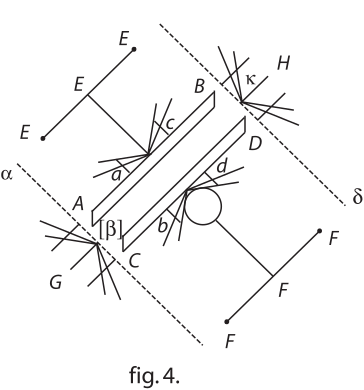
\includegraphics[width=0.46\textwidth]{images/37_3_139r4}\\\textit{[Fig. 3]}
%                        %\caption{Bildbeschreibung}
%                        \end{center}
\pstart 
\textso{Mais comme ce raisonnement n'est que }\edlabel{Maisstart}\textso{vraysemblable, il est important de venir \`{a} une experience facile, et, ce me semble, demonstrative, pour s\c{c}avoir si l'union des }\textso{corps purgez}\protect\index{Sachverzeichnis}{corps!purg\'{e}}\textso{ d'air, peut estre attribu\'{e}e au mouuement interieur du }\textso{fluide}\protect\index{Sachverzeichnis}{fluide}\textso{ ambient. Soient\linebreak(fig. 4}\footnote{\textit{In der rechten Spalte}: fig. 4 \textit{als Platzhalter für die fehlende Zeichnung.}}\edtext{}{\lemma{4}\Afootnote{\textit{Leibniz unterstreicht}: \textso{fig. 4}}}\textso{)}
%\begin{wrapfigure}{l}{0.4\textwidth}                    
    %            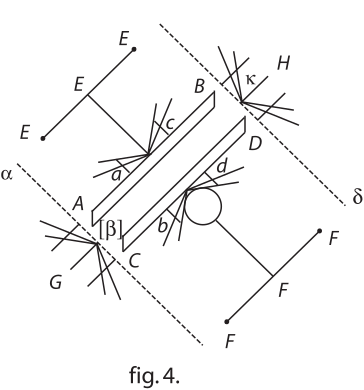
\includegraphics[width=0.4\textwidth]{images/37_3_139r4}\\\textit{[Fig. 3]}
                        %\caption{Bildbeschreibung}
        %                \end{wrapfigure}
                        %@ @ @ Dies ist eine Abstandszeile - fuer den Fall, dass mehrere figures hintereinander kommen, ohne dass dazwischen laengerer Text steht. Dies kann zu einer Fahlermeldung fuehren. @ @ @ \\
                    \textso{deux placques}\protect\index{Sachverzeichnis}{deux placques}\textso{ }\textit{\textso{AB}}\textso{ et }\textit{\textso{CD}}\textso{ la superieure }\textit{\textso{AB }}\edtext{\textso{fixe au bout inferieur }\textit{\textso{ac}}\textso{ d'un}}{\lemma{\textso{fixe}}
                    \Afootnote{ \textit{ (1) }\ \textso{\`{a} un} \textit{ (2) }\ \textso{au bout inferieur }\textit{\textso{ac}} \textso{d'un} \textit{ L}}}
 %\linebreak
 \textso{bâton }\edtext{\textso{immobile}}{\lemma{\textso{b\^{a}ton}}\Afootnote{ \textit{ (1) }\ \textso{de fer} \textit{ (2) }\ \textso{immobile} \textit{ L}}}
\textit{\textso{ac}}\textso{ l'inferieu\-re }\textit{\textso{CD}}\textso{ couch\'{e}e librement sur le bout superieur }\textit{\textso{bd}}\textso{ du}\linebreak \textso{bâton immobile }\textit{\textso{bd}}\textso{ en sorte que leur distance }\textit{\textso{AC}}\textso{, }\textit{\textso{BD}}\textso{ soit autant petite qu'il est possible, et qu'\`{a} peine on puisse voir le jour \`{a} travers. Je dis qu'alors la liqueur ambiente de l'espace }\textit{\textso{EACFDBE}}\textso{ so\^{u}slevant la placque inferieure }\textit{\textso{CD}}\textso{ la joindra \`{a} la superieure }\textit{\textso{AB}}\textso{ s'il est }\edtext{\textso{vray}}{\lemma{}\Afootnote{\textso{vray} \textit{ erg.} \textit{ L}}}\textso{ que }\edtext{\textso{le mouuement interieur de cette liqueur seroit capable de so\^{u}tenir la m\^{e}me placque inferieure si elle estoit d\'{e}ja effectivement jointe}}{\lemma{\textso{que}}\Afootnote{ \textit{ (1) }\ \textso{la m\^{e}me placque estant d\'{e}ja joincte} \textit{ (2) }\ \textso{le} [...] \textso{inferieure}  \textbar\ \textso{\textit{CD}} \textit{ gestr.}\ \textbar\ \textso{si} [...] \textso{jointe} \textit{ L}}}\textso{ \`{a} la superieure.}\edlabel{Maisend}\edtext{}{\lemma{\textso{Mais} [...] \textso{superieure.}}\xxref{Maisstart}{Maisend}\Afootnote{\textit{Markierung am Rand}}} Pourveu que la distance \textit{AC} ou \textit{BD} ne soit point considerable \edtext{\`{a} l'\'{e}gard de}{\lemma{}\Afootnote{\`{a} l'\'{e}gard de \textit{ erg.} \textit{ L}}} la longueur ou largeur des placques, c'est \`{a} dire de la ligne \textit{AB} ou \textit{CD}. La demonstration de cela est ais\'{e}e. Car soit \`{a} present la ligne \textit{AB} transport\'{e}e en $\alpha\beta$ et la ligne \textit{CD} en $\kappa\delta$ \`{a}fin que la distance \textit{AC} puisse estre prise dans la ligne $\alpha\beta$, et la distance \textit{BD} dans la ligne $\kappa\delta$. Et soient prises dans la ligne \textit{AB}, la partie \textit{ac} \'{e}galle \`{a} la distance \textit{AC} et dans la ligne \textit{CD} la partie \textit{bd} \'{e}galle \`{a} la distance \textit{BD} et soit \textit{ac} (\textit{AC}) ou \textit{bd} (\textit{BD}) une partie peu considerable, par exemple la centi\`{e}me de la ligne \textit{AB}, ou \textit{CD}, il est constant que la placque \textit{CD} sera pouss\'{e}e vers la placque \textit{AB} par une infinit\'{e} de coups du mouuement de la liqueur qui \edtext{vont}{\lemma{qui}\Afootnote{ \textit{ (1) }\ tombent \textit{ (2) }\ vont \textit{ L}}} de \textit{FFF} vers \textit{CD}. Voyons \`{a} present s'il y a autant de coups qui la repoussent, mais il s'en faut bien. Car tous les coups contraires, qui viennent d'\textit{EEE} vers \textit{AB} ne touchent pas la placque \textit{CD} estant so\^{u}ten\"{u}s par la placque  \textit{AB} \edtext{et on peut}{\lemma{\textit{AB}}\Afootnote{ \textit{ (1) }\ de sorte qu \textit{ (2) }\ et on peut \textit{ L}}} dire generalement, qu'outre ceux qui viennent de \textit{FFF} et qui la poussent vers la placque \edtext{superieure, il}{\lemma{superieure}\Afootnote{\textbar\ \textit{CD} \textit{ gestr.}\ \textbar\ , il \textit{ L}}} n'y a point d'autres qui \edtext{tombent sur la}{\lemma{qui}\Afootnote{ \textit{ (1) }\ la rep \textit{ (2) }\ tombent sur la \textit{ L}}} placque inferieure \textit{CD} (sa largeur ou glaive n'estant pas considerable, et si elle le seroit, les coups qui tombent la dessus ne contribuant rien ny \`{a} pousser ny \`{a} repousser) que ceux qui entrent entre \textit{AC} et \textit{BD}. Mais tous les coups qui entrent par l\`{a}, ne peuuent estre que deux fois ceux qui tombent sur \textit{bd}. Puisque \textit{BD} est \'{e}gal \`{a} \textit{bd} et \textit{AC} \`{a} \textit{BD} aussi bien que \textit{bd} et que la liqueur estant uniforme, il faut que tant de coups tombent sur \textit{AC} ou \textit{BD} que sur \textit{bd} la ligne \textit{CD} estant transport\'{e}e \edtext{par imagination}{\lemma{par}\Afootnote{imagination \textit{ erg.} \textit{ L}}} en $\kappa\delta$, et \textit{bd} avec, en \textit{BD}.
[139 v\textsuperscript{o}] Donc les coups qui tombent sur \textit{bd}: \edtext{centi\`{e}me partie de la ligne \textit{CD}}{\lemma{}\Afootnote{centi\`{e}me partie de la ligne \textit{CD} \textit{ erg.} \textit{ L}}} estant la centi\`{e}me partie de tous les coups qui tombent sur la ligne \edtext{entiere}{\lemma{ligne}\Afootnote{ \textit{ (1) }\ interieur \textit{ (2) }\ entiere \textit{ L}}} \textit{CD}. Il s'ensuit que les coups qui tombent sur \textit{AC} et \textit{BD} \edtext{pris ensemble lesquels sont seuls capables de repousser}{\lemma{\textit{BD}}\Afootnote{ \textit{ (1) }\ ensemble \textit{ (2) }\ pris [...] repousser \textit{ L}}}, soyent deux fois la centi\`{e}me partie des coups qui poussent, c'est \`{a} dire qui tombent sur la ligne \textit{CD} et par consequent les coups qui poussent la placque \textit{CD} vers la placque \textit{AB} surmonteront sans peine ceux qui pourroient repousser, et dont la quantit\'{e} n'est point du tout considerable, \edtext{n'estant au plus \`{a} l'\'{e}gard}{\lemma{n'estant}\Afootnote{ \textit{ (1) }\ qu'\`{a} la \textit{ (2) }\  au plus \`{a} l'\'{e}gard \textit{ L}}} de ceux qui poussent, que comme 2. \`{a} 100. en nostre exemple. Je dis: \textso{au plus,} parce qu'en effect la plus grande partie de ceux m\^{e}mes qui tombent sur \textit{AC}, et \textit{BD} est de nul usage pour repousser la placque \textit{CD}. Car du cost\'{e} \edtext{\textit{BD} (le m\^{e}me s'entend de l'autre cost\'{e} \textit{AC})}{\lemma{\textit{BD}}\Afootnote{ \textit{ (1) }\ premierement \textit{ (2) }\ (le [...] \textit{AC}) \textit{ L}}} la ligne \edtext{du coup}{\lemma{}\Afootnote{du coup \textit{ erg.} \textit{ L}}} \textit{HG} et toutes les autres perpendiculaires \`{a} $\kappa\delta$ passent entre les deux placques\protect\index{Sachverzeichnis}{deux placques} sans rien faire; par apres: les \edtext{vagues}{\lemma{les}\Afootnote{ \textit{ (1) }\ coups \textit{ (2) }\ vagues \textit{ L}}} qui entrent entre \textit{H} et $\delta$ frappant directement la superficie interieure de la placque immobile \textit{AB} ne contribuent rien \`{a} repousser l'inferieure \textit{cd} si non peut estre par reflexion\protect\index{Sachverzeichnis}{r\'{e}flexion}; \edtext{il restent}{\lemma{reflexion;}\Afootnote{ \textit{ (1) }\ ce sont \textit{ (2) }\ il restent \textit{ L}}} donc celles seulement qui viennent entre $\kappa$ et \textit{H}\edtext{}{\lemma{\textit{H}}\Afootnote{ \textbar\ et \textit{c} \textit{ gestr.}\ \textbar\ . On \textit{ L}}}. On dira peut-estre, par un esprit de chicane, que celles qui viennent d'entre $\kappa$ et \textit{H} quoyque peu en nombre sont les plus considerables en forces, venant de haut en bas, et portant un choc\protect\index{Sachverzeichnis}{choc} redoubl\'{e} par la pesanteur naturelle de la liqueur. Mais cet avantage est icy de peu de consequence, car sans insister sur ce que tous les coups qui doiuuent so\^{u}tenir la \edtext{placque}{\lemma{la}\Afootnote{ \textit{ (1) }\ table \textit{ (2) }\ placque \textit{ L}}} inferieure libre, attach\'{e}e \`{a} la superieure fixe, sont de bas \textit{F} en haut \textit{CD} contre le mouuement naturel\protect\index{Sachverzeichnis}{mouvement!naturel} des corps pesants; il faut seulement considerer l'exemple des placques; suspend\"{u}es dans le vuide\protect\index{Sachverzeichnis}{vide}, car la pesanteur \edtext{de tout l'air ou matiere plus subtile que l'air}{\lemma{pesanteur}\Afootnote{ \textit{ (1) }\ de toute la matiere \textit{ (2) }\ de tout l'air  \textit{(a)}\ ou autre matiere \textit{(b)}\ ou [...] l'air \textit{ L}}} qui reste la dedans est presqu'insensible, et peut sans scrupule estre cont\'{e}e pour rien; et on pretend neantmoins que le mouuement interieur dans les parties de ce fluide\protect\index{Sachverzeichnis}{fluide} soit capable de so\^{u}tenir un poids\protect\index{Sachverzeichnis}{poids} de trois liures et d'avantage.
\pend 